% 由 tutorial.tex 自动拆分为第 15 章
\chapter{训练方法：从 SGD 到 AdamW}
前面所有推导只解决了"梯度怎么算"。这一节解决"拿到梯度后怎么走"。

\section{为什么普通梯度下降不够}

设 $\theta\in\mathbb{R}^2$、损失 $f=\tfrac12(x^2+\kappa y^2)$，$\kappa=50$。
梯度下降的迭代是
\begin{equation}
  \theta_{t+1}=\theta_t-\eta\nabla f(\theta_t)
  \;\Longrightarrow\;
  x_{t+1}=(1-\eta)x_t,\quad y_{t+1}=(1-50\eta)y_t .
\end{equation}
稳定性要求 $|1-50\eta|<1\Rightarrow\eta<0.04$；而 $x$ 方向的收敛速度是 $(1-\eta)^t$，
在 $\eta=0.018$ 时要 $250$ 步才能缩小到 $10^{-2}$。\textbf{一个学习率被最陡方向绑架}，
这就是病态（ill-conditioned）问题。

本模型实测：各层梯度范数从 $12$ 到 $70$，相差近 $6$ 倍；同一层内部逐元素还能差更多。

\section{动量}

\begin{equation}
  v_t=\beta v_{t-1}+g_t,\qquad \theta_t=\theta_{t-1}-\eta v_t .
\end{equation}
展开得 $v_t=\sum_{k\le t}\beta^{t-k}g_k$，即梯度的指数加权和。
陡方向的正负震荡被平均掉，平方向的分量被累积。有效学习率约为 $\eta/(1-\beta)$——
$\beta=0.9$ 时放大约 $10$ 倍，所以动量的 $\eta$ 必须相应调小。

\section{RMSProp：逐参数步长}

\begin{equation}
  v_t=\beta_2v_{t-1}+(1-\beta_2)g_t^2,\qquad
  \theta_t=\theta_{t-1}-\eta\frac{g_t}{\sqrt{v_t}+\varepsilon} .
\end{equation}
分母是梯度平方的滑动平均：梯度一直大的参数步子自动变小，梯度小的自动变大。
\textbf{本模型第一步实测}：SGD 下 \texttt{w\_head} 的步长是 \texttt{l1.W\_qkv} 的
$31$ 倍；RMSProp/Adam 下两者完全相同（都是 $\eta$）。

\section{Adam 与偏差修正}

\begin{align}
  m_t&=\beta_1m_{t-1}+(1-\beta_1)g_t, &
  v_t&=\beta_2v_{t-1}+(1-\beta_2)g_t^2,\\
  \hat m_t&=\frac{m_t}{1-\beta_1^t}, &
  \hat v_t&=\frac{v_t}{1-\beta_2^t},\\
  \theta_t&=\theta_{t-1}-\eta\,\frac{\hat m_t}{\sqrt{\hat v_t}+\varepsilon}. &&
\end{align}

\begin{quote}
\textbf{为什么必须做偏差修正}：$m_0=v_0=0$，所以 $m_1=(1-\beta_1)g_1$、$v_1=(1-\beta_2)g_1^2$，
都被缩放了。$t=1$ 时 $1-\beta_2^t=0.001$——不修正的话分母 $\sqrt{v}$ 小 $\sqrt{1000}\approx31.6$ 倍，
步长会被放大 $31.6$ 倍，前几步直接炸掉。修正后 $m_1/(1-\beta_1)=g_1$、$v_1/(1-\beta_2)=g_1^2$，
第一步的步长正好是 $\eta$（逐元素符号方向）。
\end{quote}

\section{AdamW：解耦权重衰减}

Adam 加 L2 正则的做法是把 $\lambda\theta$ 塞进梯度：
\begin{equation}
  g_t\leftarrow g_t+\lambda\theta_{t-1}
  \ \Rightarrow\ \theta_t=\theta_{t-1}-\eta\frac{\hat m_t}{\sqrt{\hat v_t}+\varepsilon}.
\end{equation}
问题是 $\lambda\theta$ 也进了二阶矩 $v_t$，于是\textbf{衰减被自适应步长归一化了}：
梯度大的参数衰减得反而少。AdamW 把衰减单独拿出来：
\begin{equation}
  \theta_t=(1-\eta\lambda)\,\theta_{t-1}-\eta\frac{\hat m_t}{\sqrt{\hat v_t}+\varepsilon},
\end{equation}
每个参数按同一比例缩小。并且\textbf{有一类参数不该衰减}：LayerNorm 的 $\gamma,\beta$、
位置编码、所有 bias——衰减它们会破坏归一化与偏置的语义。

\section{学习率调度}

本课用余弦退火：
\begin{equation}
  \eta_e=\frac{\eta_{\max}}{2}\Big(1+\cos\frac{\pi e}{E}\Big),
  \qquad \eta_{\max}=2\times10^{-3},\ E=8 .
\end{equation}
前期大步探索，后期小步精修。

\section{实测对比}

同一模型、同一初始化、同一批数据顺序，各训 $3$ 个 epoch：

\begin{center}
\small
\begin{tabular}{@{}lcccc@{}}
\toprule
优化器 & 学习率 & 首轮平均损失 & 三轮后 & 结论 \\
\midrule
AdamW & $2\times10^{-3}$ & $7.04$ & $\mathbf{0.047}$ & 收敛 \\
Adam & $2\times10^{-3}$ & $7.04$ & $0.047$ & 与本课等价 \\
RMSProp & $2\times10^{-3}$ & $57.6$ & $0.043$ & 收敛但首轮更抖 \\
SGD & $10^{-3}$ & $44.2$ & $4.47$ & 慢 \\
Momentum & $10^{-3}$ & $63.5$ & $59.9$ & 有效学习率偏大，震荡 \\
SGD & $2\times10^{-2}$ & $70.7$ & $72.0$ & \textbf{发散} \\
\bottomrule
\end{tabular}
\end{center}

\begin{figure}[htbp]
\centering
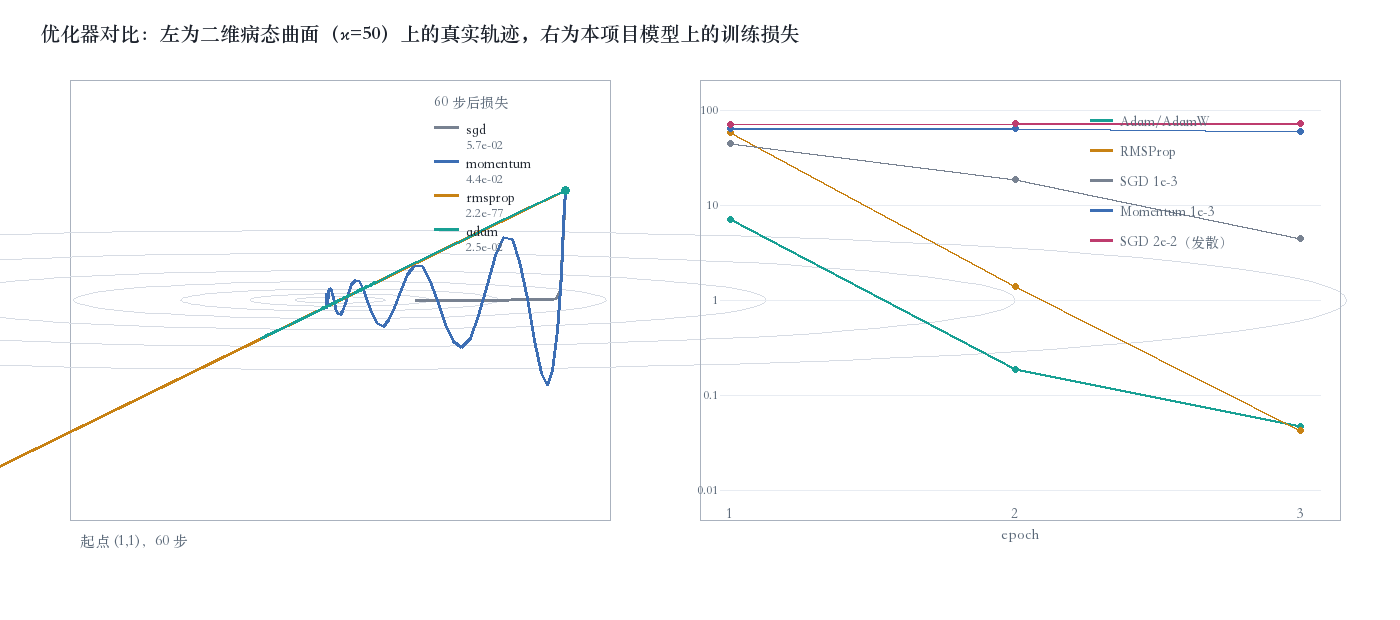
\includegraphics[width=0.96\linewidth]{fig_optim.png}
\caption{左：二维病态曲面（$\kappa=50$）上四种优化器的真实轨迹，60 步后损失分别为
SGD $5.7\times10^{-2}$、Momentum $4.4\times10^{-2}$、RMSProp $2\times10^{-77}$、Adam $2.5\times10^{-2}$。
右：本模型上五种优化器的训练损失（Adam 与 AdamW 完全重合）。}
\end{figure}

